\documentclass[journal]{IEEEtran}
\usepackage{cite}
\usepackage{amsmath,amssymb}
\usepackage{graphicx}
\usepackage{booktabs}
\usepackage{url}
\usepackage[hidelinks]{hyperref}

\graphicspath{{../figures/}}

\begin{document}

\title{Cut-Dependent Inference-Time Aggregation for C-MAPSS Remaining Useful Life:
When Learned Gating Helps and When It Does Not}

\author{Anonymous Authors}

\maketitle

\begin{abstract}
Multi-window aggregation is a common inference-time step for remaining useful
life (RUL) prediction, yet its benefit is usually reported as a single average
over the engine life. We ask whether that benefit is uniform, and we find that it
is not. On a frozen C-MAPSS backbone, a learned gate (LTAG) improves official
test RMSE over a single-window baseline on all four subsets (15/15 seed-subset
wins; mean improvement 0.391 cycles). The same gate is not the best aggregator on
a five-cut validation average: a context-aware residual calibration and a linear
stack are stronger there. A cut-wise analysis resolves the apparent conflict.
Calibration methods are stronger at early cuts (0.40--0.55), where errors are
large; near end-of-life (0.85--0.95), LTAG is competitive with or better than the
calibration baselines. The validation mean is therefore dominated by early cuts
and is not a reliable proxy for the end-of-life test. We also revisit a
measurement-model sensor-reconstruction front-end: with fair backtracked hold and
median baselines, it only helps on stuck sensors and is not a general component.
The paper's contribution is a cut-controlled evaluation protocol and the
empirical finding that learned gating and post-hoc calibration win different
parts of the engine life.

\end{abstract}

\begin{IEEEkeywords}
remaining useful life, C-MAPSS, multi-window aggregation, learned gating,
calibration, sensor reconstruction.
\end{IEEEkeywords}

\section{Introduction}
\label{sec:intro}

Remaining useful life (RUL) models are usually judged by their accuracy near the
end of an engine's life, because that is when a maintenance decision is made.
Yet many models produce a sequence of predictions from overlapping windows and
aggregate them with a fixed rule or a learned gate. The aggregation step is often
evaluated on a mixture of early and late cuts, and a single average can hide a
change in ranking across the engine life.

This paper asks a narrow question: \emph{does the benefit of multi-window
aggregation depend on where in the engine life the prediction is made?} We study
the question on the C-MAPSS benchmark \cite{saxena2008} with a frozen backbone and
a fixed evaluation protocol. The protocol separates five cut fractions
(0.40, 0.55, 0.70, 0.85, 0.95), keeps validation and test engines disjoint, and
reports engine-mean and pooled RMSE separately.

Our first result is positive for a learned gate. LTAG aligns the predictions of
several windows to the current cut and learns a gate that mixes the age-aligned
median with the single-window prediction. On the frozen B0 backbone, LTAG lowers
official test RMSE on all four subsets, with 15/15 seed-subset wins and a mean
improvement of 0.391 cycles (Table~\ref{tab:test}).

Our second result is a boundary. On a validation average over all five cuts, two
simple alternatives are stronger: a context-aware residual calibration
(K1-Calib) and a linear stack (LS-ctx). This is not a small effect: K1-Calib and
LS-ctx beat LTAG on all four subsets (Table~\ref{tab:validation}). A naive reading
would reject LTAG. A cut-wise decomposition shows why the two results are
compatible. The calibration methods are much stronger at early cuts, where the
error is large and the validation mean is dominated by those cuts. At 0.85--0.95,
LTAG is competitive with or better than the calibration methods
(Table~\ref{tab:cutwise}, Figure~\ref{fig:cutwise}). The official test uses one
window per engine near end-of-life, so it is closer to the late cuts than to the
validation mean.

Our third result is negative for a measurement-model front-end. An earlier
sensor-reconstruction module (RHSE-TSH) looked effective against a last-value
baseline. With fair backtracked hold and median baselines that use only observed
data, the reconstruction matches or loses on bias and drift and only helps on
stuck sensors (Table~\ref{tab:rhse}). We therefore remove it from the method and
keep the finding as a boundary.

The contributions are:
\begin{enumerate}
\item A cut-controlled evaluation protocol for multi-window RUL aggregation that
reports engine-mean and pooled RMSE separately and never mixes estimators.
\item A positive test result for LTAG on a frozen backbone: 15/15 seed-subset
wins, mean test RMSE improvement 0.391 cycles (Section~\ref{sec:exp}).
\item A cut-wise diagnosis showing that calibration wins early cuts while LTAG
is competitive or better near end-of-life; the validation mean is not a proxy
for the end-of-life test (Section~\ref{sec:cutwise}).
\item A negative result for measurement-model sensor reconstruction under fair
temporal baselines; the module is retained only as a limitation
(Section~\ref{sec:rhse}).
\end{enumerate}

We do not claim a new state of the art. The paper's value is the cut-controlled
evidence and the boundary: a learned gate can be the right choice at end-of-life
even when a simple calibration wins the all-cut average.

The rest of the paper describes the protocol (Section~\ref{sec:setup}), the LTAG
method (Section~\ref{sec:method}), the test and validation results
(Section~\ref{sec:exp}), the cut-wise analysis (Section~\ref{sec:cutwise}), the
negative sensor-reconstruction result (Section~\ref{sec:rhse}), and the
limitations (Section~\ref{sec:conclusion}).

\section{Related Work}
\label{sec:related}

\paragraph{C-MAPSS and RUL backbones.}
The C-MAPSS turbofan benchmark \cite{saxena2008} provides run-to-failure
trajectories for four subsets with different operating conditions and fault
modes. Most recent work trains a sequence model on the sensor trajectories and
predicts a capped RUL target. Reported gains are usually measured on a single
test window per engine, and the aggregation of multiple overlapping windows is
often treated as an implementation detail. Our protocol keeps the backbone frozen
and varies only the inference-time aggregation, so the comparison is not
confounded by backbone training.

\paragraph{RUL with uncertainty and domain shift.}
Evidential and domain-adaptation approaches model uncertainty or incomplete
degradation \cite{hou2025}; quantile and state-space approaches produce
distributional RUL estimates \cite{frizzo2025}; scientific machine learning
combines physics and data for engine health management \cite{barry2026}; and
survival-based aging models link degradation to RUL \cite{srinivasan2026}. These
lines improve the predictor itself. Our question is complementary: given a fixed
predictor, when does multi-window aggregation help, and when does a simple
post-hoc calibration suffice?

\paragraph{Aggregation and calibration.}
Fixed rules (mean, median, last value) and learned gates are common ways to
combine overlapping predictions. Post-hoc calibration (a linear or residual map
from predictions and context to the target) is equally common in deployment.
Calibration and reliability diagnostics have also been studied for RUL under
operating-regime shift \cite{yang2026}, as have conformal and similarity-based
interval methods \cite{busico2026,barber2023} and business-aware uncertainty
estimates \cite{frizzo2026}. These lines calibrate intervals or reliability;
they do not compare point-aggregation rankings across cuts.
The two families are rarely compared under the same cut protocol. We compare
them on the same frozen features, with the same engine-disjoint folds, and
report where each family wins. The result is a cut-dependent ranking rather than
a single winner.

\paragraph{Sensor-fault reconstruction.}
Measurement-model reconstruction uses a low-rank model of healthy sensor
correlations to replace a flagged sensor. It is attractive because it is
interpretable and can run online. The risk is that a temporal hold or median
baseline can recover the same signal without a model. We therefore compare the
reconstruction against fair backtracked baselines that use only observed data,
not against a weak last-value baseline. This is the comparison that removes the
apparent advantage on bias and drift.

\section{Protocol and Setup}
\label{sec:setup}

\subsection{Data and splits}

We use the four C-MAPSS subsets \cite{saxena2008}: FD001 (one condition, one
fault mode), FD002 (six conditions, one fault mode), FD003 (one condition, two
fault modes), and FD004 (six conditions, two fault modes). The RUL target is
capped at 125 cycles. Engines are split into training and validation engines;
validation engines are never used for fitting, early stopping, or model
selection. The official test engines are sealed until the frozen configuration
is fixed; we do not use test labels for any choice in this paper.

For validation we evaluate five cut fractions of each engine's life:
0.40, 0.55, 0.70, 0.85, and 0.95. Each cut produces one prediction per engine.
The official test provides one window per engine near end-of-life, so the 0.95
cut is the closest validation analogue. This distinction is central to the
analysis in Section~\ref{sec:cutwise}.

\subsection{Backbone and baselines}

The backbone is a frozen DSPT-style model (B0) trained under a fixed protocol:
two layers, model width 64, dropout 0.2, FP32, 40 epochs, patience 12, batch
size 512, learning rate $10^{-3}$, and weight decay $10^{-4}$. We do not retrain
the backbone for any experiment in this paper. The single-window prediction from
this backbone is denoted K1. The median of age-aligned windows is denoted Median.

\subsection{Estimators}

Two estimators are reported and never mixed:
\begin{itemize}
\item \emph{Engine-mean RMSE}: compute RMSE per engine, then average over
engines. This gives every engine equal weight.
\item \emph{Pooled RMSE}: pool all windows and compute one RMSE. This weights
engines by their number of windows.
\end{itemize}
The identity $\mathrm{pooled}^2-\mathrm{engine\_mean}^2=\mathrm{Var}_e(\mathrm{RMSE}_e)$
holds when every engine has the same number of windows; we use it as a
consistency check. The official test has one window per engine, so the two
estimators coincide there.

For paired comparisons we resample engines with replacement (10{,}000 draws) and
report the mean difference, its 95\% confidence interval, and a one-sided
$p$-value. When multiple seeds are available, predictions are averaged within an
engine before resampling, so the unit of replication is the engine, not the seed.

\subsection{Reproducibility note}

The Phase~2 experiments in the broader project used a worktree code lock rather
than the original commit; the lock file and the current worktree hashes are
retained in the repository. The LTAG experiments in this paper use the frozen
B0 checkpoint and the feature table described in Section~\ref{sec:method}; no
test-time tuning is performed.

\section{Method}
\label{sec:method}

\subsection{Age-aligned windows}

For an engine at cut $c$, let $t_0=c-1$ be the index of the most recent cycle.
For a window lag $\Delta$ and offset $j$, the window ends at $t_j=t_0-j\Delta$.
The backbone prediction for that window is $p_j$. Because the window is older
than the cut, its prediction refers to an earlier cycle. We align it to the cut:
\begin{equation}
a_j = p_j + j\Delta .
\label{eq:align}
\end{equation}
The aligned predictions $\{a_j\}_{j=0}^{K-1}$ are the inputs to the aggregator.
For $K=1$, $a_0=p_0=K1$; for $K=3$ and $\Delta=5$ we use offsets $j=0,1,2$.

\subsection{Features}

The aggregator uses eleven features: the single-window prediction $p_0$, the
aligned median $p_{\mathrm{med}}$, the aligned mean $p_{\mathrm{mean}}$, the
aligned standard deviation $p_{\mathrm{std}}$, the median absolute deviation
(MAD), the shift $p_{\mathrm{med}}-p_0$, the regime distance, the cap indicator,
the current cut normalized by 250, and the observed history length normalized by
70. The lifetime fraction $c/n$ is deliberately excluded: the true lifetime $n$
is not observable at test time. The cap indicator is computed from the model
outputs ($p_0\ge 124.5$ or $p_{\mathrm{med}}\ge 124.5$), not from the true RUL.

\subsection{Learned gate}

LTAG is a two-layer MLP with GELU activation and a sigmoid output:
\begin{equation}
g(x)=\sigma\!\left(W_2\,\mathrm{GELU}(W_1 x+b_1)+b_2\right),
\end{equation}
with the last layer initialized to zero, so the gate starts at $g=0.5$. The
prediction is
\begin{equation}
\hat y = g\,p_{\mathrm{med}} + (1-g)\,p_0 .
\label{eq:gate}
\end{equation}
The gate is trained with a censored hinge loss on the capped target,
\begin{equation}
\ell(\hat y,y)=
\begin{cases}
\max(0,\hat y-y), & y<125,\\
\max(0,\hat y-125), & y=125,
\end{cases}
\end{equation}
which avoids penalizing a prediction above the cap when the true RUL is capped.
Training uses AdamW, learning rate $10^{-3}$, weight decay $10^{-3}$, 300 epochs,
and five engine-disjoint folds (GroupKFold by subset and engine). Validation
engines are not used in any fold.

\subsection{Calibration baselines}

We compare two post-hoc calibrators on the same features. K1-Calib is a residual
MLP that predicts $\hat y=p_0+r(x)$, where $r$ is a two-layer MLP with zero-init
last layer and the input contains only $p_0$ and context (regime distance, cap,
cut, history). LS-ctx is a ridge regression on
$[p_0,p_{\mathrm{med}},\text{context}]$. Both are trained on the training engines
and applied to validation engines; neither sees test labels.

The distinction between LTAG and the calibrators is deliberate. LTAG learns a
\emph{gate} between two existing predictions; K1-Calib learns an additive
correction to $p_0$; LS-ctx learns a linear map. If a calibrator matches LTAG,
the gate is not necessary. Section~\ref{sec:cutwise} shows that the answer
depends on the cut.

\section{Experiments}
\label{sec:exp}

\subsection{Official test}

Table~\ref{tab:test} reports the frozen B0 test RMSE. Each test engine has one
window. LTAG lowers RMSE on all four subsets and on every seed: 6/6 on FD001 and
3/3 on each of FD002--FD004, for 15/15 seed-subset wins. The mean improvement is
0.391 cycles, from 13.421 to 12.995 on FD001, 11.514 to 11.352 on FD002, 12.979
to 12.323 on FD003, and 13.031 to 12.710 on FD004. Figure~\ref{fig:test} shows
the per-subset bars and the individual seed points.

\begin{table*}[t]
\centering
\caption{Frozen B0 official test RMSE (one window per engine; lower is better).
LTAG improves over K1 on every subset and every seed (15/15).}
\label{tab:test}
\begin{tabular}{lcccccc}
\toprule
Subset & Seeds & K1 & LTAG & Median & $\Delta$(K1$-$LTAG) & LTAG wins \\
\midrule
FD001 & 6 & 13.421 & \textbf{12.995} & 13.364 & +0.426 & 6/6\\
FD002 & 3 & 11.514 & \textbf{11.352} & 11.803 & +0.162 & 3/3\\
FD003 & 3 & 12.979 & \textbf{12.323} & 13.002 & +0.656 & 3/3\\
FD004 & 3 & 13.031 & \textbf{12.710} & 13.601 & +0.321 & 3/3 \\
\midrule
Mean & -- & -- & -- & -- & +0.391 & 15/15 \\
\bottomrule
\end{tabular}
\end{table*}


\subsection{Validation controls}

Table~\ref{tab:validation} reports the five-cut validation average. The
single-window baseline K1 is 12.094/11.527/12.793/13.608 on FD001--FD004.
Median is better on FD001 (11.429) but worse on the other three subsets. LTAG is
11.334/11.210/12.372/13.522, an improvement over K1 on all four subsets.

The calibration baselines are stronger on this average. K1-Calib reaches
10.931/10.970/12.129/12.839, and LS-ctx reaches 10.150/10.604/12.033/13.080.
Both beat LTAG on all four subsets. A gate that mixes two existing predictions is
therefore not the best aggregator when all cuts are weighted equally.

This is the point at which a single-number comparison would reject LTAG. The next
section shows that the average hides a change in ranking across the engine life.

\begin{table}[t]
\centering
\caption{Validation engine-mean RMSE (observable features; 5 cuts; seeds
101/202/303, FD001 adds 404/505/606). Lower is better.}
\label{tab:validation}
\begin{tabular}{lcccc}
\toprule
Arm & FD001 & FD002 & FD003 & FD004 \\
\midrule
K1 & 12.094 & 11.527 & 12.793 & 13.608 \\
Median & 11.429 & 11.704 & 12.984 & 14.399 \\
LTAG & 11.334 & 11.210 & 12.372 & 13.522 \\
Global-g & 11.503 & 11.234 & 12.622 & 13.661 \\
K1-Calib & 10.931 & 10.970 & 12.129 & 12.839 \\
Linear-Stack & 10.150 & 10.604 & 12.033 & 13.080 \\
LTAG-noMW & 11.299 & 11.186 & 12.526 & 13.583 \\
\bottomrule
\end{tabular}
\end{table}


\begin{figure}[t]
\centering
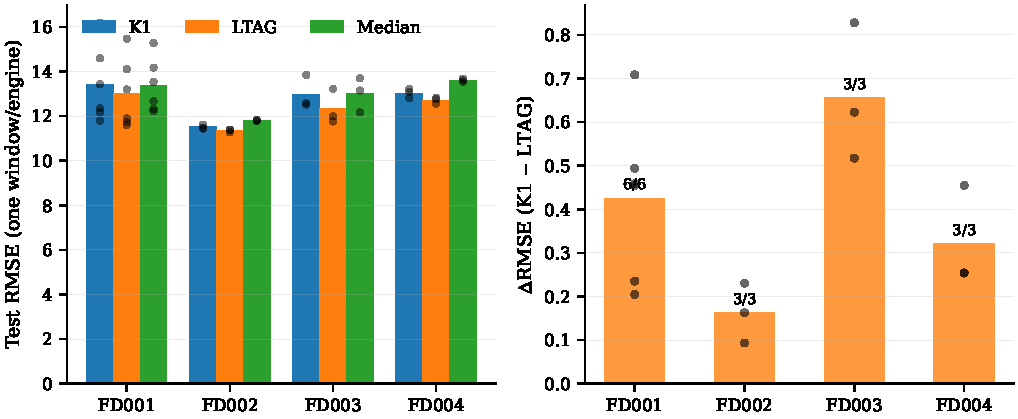
\includegraphics[width=0.48\textwidth]{fig2_test.pdf}
\caption{Frozen B0 test RMSE (one window per engine). Bars are subset means; dots
are individual seeds. LTAG is lower than K1 on all four subsets (15/15).}
\label{fig:test}
\end{figure}

\subsection{Ensemble control}

Averaging three seeds (101/202/303) gives Ens3-K1 11.005/11.231/11.828/13.342 and
Ens3-LTAG 10.292/10.937/11.410/13.228. The gate still helps on top of the
ensemble (4/4), but the ensemble itself closes much of the gap. Ens3-LTAG remains
below LS-ctx on all four subsets (9.256/10.483/11.026/12.903), so the ensemble
control does not rescue the gate as a universal aggregator.

\section{Cut-Dependent Analysis}
\label{sec:cutwise}

\subsection{Ranking changes with the cut}

Table~\ref{tab:cutwise} reports engine-mean RMSE at each of the five cuts.
At 0.40, LS-ctx is much better than LTAG on every subset (differences
$-4.170/-1.548/-1.239/-0.904$). At 0.55 the advantage shrinks but remains
negative on all four subsets. At 0.70 the two methods are close. At 0.85 and
0.95 the sign reverses on FD001, FD002, and FD004: LTAG is better than LS-ctx.
The crossover is the source of the apparent conflict between
Tables~\ref{tab:test} and~\ref{tab:validation}. The validation average is
dominated by the early cuts, where the error is large; the test is a single
end-of-life window.

\begin{figure*}[t]
\centering
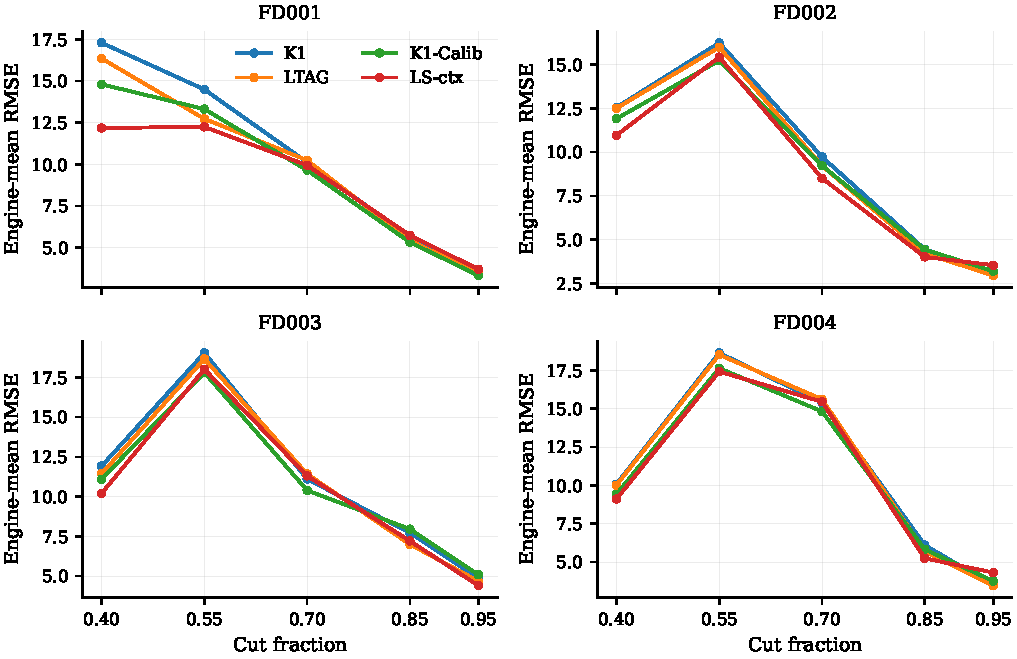
\includegraphics[width=0.95\textwidth]{fig1_cutwise.pdf}
\caption{Cut-wise engine-mean RMSE for K1, LTAG, K1-Calib, and LS-ctx. Calibration
is stronger at early cuts; LTAG is competitive or better near end-of-life.}
\label{fig:cutwise}
\end{figure*}

\begin{table*}[t]
\centering
\caption{Cut-wise validation engine-mean RMSE. LS-ctx is stronger at early cuts;
LTAG is competitive or better at 0.85--0.95. The last column is LS$-$LTAG
(positive = LTAG better).}
\label{tab:cutwise}
\small
\begin{tabular}{llcccccc}
\toprule
Subset & Cut & K1 & LTAG & K1-Calib & LS-ctx & LS$-$LTAG \\
\midrule
FD001 & 0.40 & 17.283 & 16.345 & 14.794 & 12.175 & -4.170 \\
FD001 & 0.55 & 14.485 & 12.724 & 13.308 & 12.243 & -0.481 \\
FD001 & 0.70 & 10.119 & 10.236 & 9.644 & 9.934 & -0.302 \\
FD001 & 0.85 & 5.593 & 5.431 & 5.318 & 5.732 & +0.301 \\
FD001 & 0.95 & 3.473 & 3.437 & 3.322 & 3.705 & +0.267 \\
FD002 & 0.40 & 12.560 & 12.512 & 11.913 & 10.964 & -1.548 \\
FD002 & 0.55 & 16.252 & 15.997 & 15.235 & 15.434 & -0.563 \\
FD002 & 0.70 & 9.731 & 9.218 & 9.229 & 8.510 & -0.708 \\
FD002 & 0.85 & 4.446 & 4.208 & 4.429 & 4.009 & -0.199 \\
FD002 & 0.95 & 3.059 & 2.942 & 3.194 & 3.534 & +0.592 \\
FD003 & 0.40 & 11.922 & 11.440 & 11.093 & 10.200 & -1.239 \\
FD003 & 0.55 & 19.045 & 18.666 & 17.812 & 18.019 & -0.646 \\
FD003 & 0.70 & 11.107 & 11.424 & 10.393 & 11.304 & -0.120 \\
FD003 & 0.85 & 7.722 & 6.994 & 7.952 & 7.207 & +0.213 \\
FD003 & 0.95 & 4.862 & 4.671 & 5.082 & 4.395 & -0.276 \\
FD004 & 0.40 & 10.079 & 10.012 & 9.421 & 9.108 & -0.904 \\
FD004 & 0.55 & 18.644 & 18.523 & 17.643 & 17.426 & -1.097 \\
FD004 & 0.70 & 15.392 & 15.617 & 14.822 & 15.454 & -0.163 \\
FD004 & 0.85 & 6.105 & 5.690 & 5.821 & 5.240 & -0.450 \\
FD004 & 0.95 & 3.468 & 3.459 & 3.752 & 4.310 & +0.851 \\
\bottomrule
\end{tabular}
\end{table*}


\subsection{End-of-life comparison}

At cut 0.95 the best method depends on the subset: K1-Calib is best on FD001
(3.322 vs LTAG 3.437), LTAG is best on FD002 (2.942 vs 3.534 for LS-ctx) and
FD004 (3.459 vs 4.310), and LS-ctx is best on FD003 (4.395 vs 4.671). LTAG is
therefore not uniformly best: it is best on FD002 and FD004, second on FD001 and
FD003, and within 0.28 of the best in every case.

A paired engine bootstrap at 0.95 makes the direction clearer. LTAG is
significantly better than K1-Calib on FD002 ($+0.252$, CI $[0.013,0.495]$) and
FD003 ($+0.411$, CI $[0.078,0.749]$), and significantly better than LS-ctx on
FD002 ($+0.592$, CI $[0.221,0.964]$) and FD004 ($+0.851$, CI $[0.120,1.626]$).
The FD001 difference in favor of K1-Calib ($-0.115$) and the FD003 difference in
favor of LS-ctx ($-0.276$) are not significant. The late-cut evidence supports
LTAG as an end-of-life aggregator, not as a universal one.

\subsection{Per-engine view}

Figure~\ref{fig:winrate} shows the per-engine difference between LS-ctx and
LTAG. LS-ctx wins on 10/20 engines on FD001, 28/52 on FD002, 10/20 on FD003, and
28/50 on FD004. The FD001 median difference is slightly positive (LS-ctx worse),
so the mean gain of LS-ctx comes from a minority of high-error engines. This is
consistent with a tail-calibration interpretation: LS-ctx lowers the largest
errors at the cost of typical accuracy, and its advantage disappears near
end-of-life.

\begin{figure}[t]
\centering
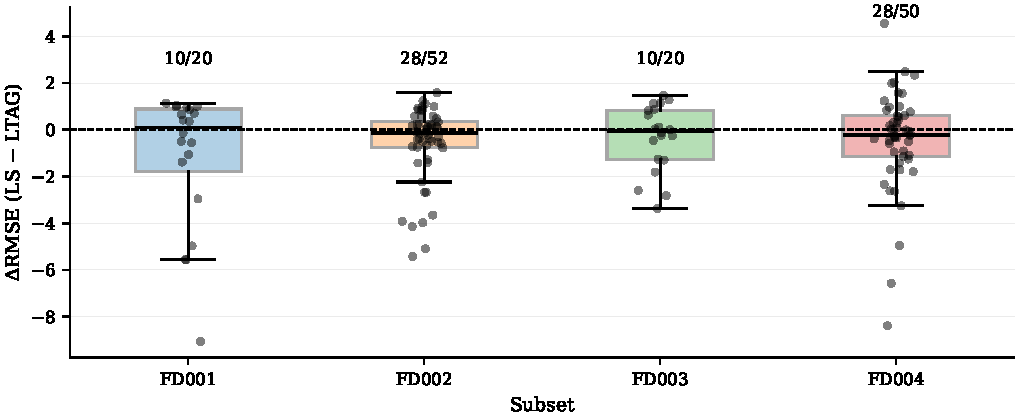
\includegraphics[width=0.48\textwidth]{fig3_winrate.pdf}
\caption{Per-engine $\Delta$RMSE (LS-ctx $-$ LTAG) on validation. Positive means
LTAG is better. LS-ctx wins on 10/20, 28/52, 10/20, and 28/50 engines; the mean
gain is driven by a minority of high-error engines.}
\label{fig:winrate}
\end{figure}

\subsection{What this means for evaluation}

A validation average over cuts is not a proxy for the end-of-life test. The same
two methods can rank in opposite orders depending on the cut composition. We
therefore recommend that multi-window RUL papers report a cut-wise table (or at
least the 0.95 cut) alongside the average. The protocol in this paper is a
minimal version of that recommendation: five cuts, engine-mean and pooled RMSE
separately, and an explicit end-of-life column.

\section{Negative Result: Sensor Reconstruction}
\label{sec:rhse}

\subsection{Motivation and baselines}

A measurement-model front-end replaces a flagged sensor with a reconstruction
from the correlations among healthy sensors. The natural baseline is a
last-value hold: keep the last observed value before the flag. That baseline is
weak on drift because it freezes the drifted value. A stronger, still fair
baseline is a backtracked hold or median that uses only observed data:
\begin{itemize}
\item R5b: hold the observed value from $t_{\mathrm{flag}}-16$;
\item R5m: take the median of the observed values in
$[t_{\mathrm{flag}}-25,t_{\mathrm{flag}}-16]$;
\end{itemize}
and replace the sensor from the flag onward. Neither baseline uses a clean
counterfactual.

We compare the reconstruction (R3, TSH plus H$\theta$) with R5b and R5m on
FD001 and FD003, for bias, drift, and stuck faults, at magnitudes 3 and onsets
0.2/0.5, over three seeds.

\begin{table*}[t]
\centering
\caption{Fair naive baselines for RHSE-TSH (3-seed mean recovery). R5b: backtracked
hold; R5m: backtracked median. R3 only passes the $\geq$0.10 gate on stuck.}
\label{tab:rhse}
\small
\begin{tabular}{llcccccc}
\toprule
Subset & Fault & Onset & R3 & R5b & R5m & R3$-$max \\
\midrule
FD001 & bias & 0.2 & 0.799 & 0.793 & 0.821 & -0.022 \\
FD001 & bias & 0.5 & 0.826 & 0.865 & 0.906 & -0.080 \\
FD001 & drift & 0.2 & 0.856 & 0.868 & 0.925 & -0.069 \\
FD001 & drift & 0.5 & 0.797 & 0.903 & 0.934 & -0.137 \\
FD001 & stuck & 0.2 & 0.737 & -0.695 & -0.202 & +0.940 \\
FD001 & stuck & 0.5 & 0.872 & 0.257 & 0.403 & +0.468 \\
FD003 & bias & 0.2 & 0.908 & 0.927 & 0.939 & -0.032 \\
FD003 & bias & 0.5 & 0.876 & 0.890 & 0.910 & -0.034 \\
FD003 & drift & 0.2 & 0.916 & 0.853 & 0.921 & -0.005 \\
FD003 & drift & 0.5 & 0.772 & 0.760 & 0.797 & -0.025 \\
FD003 & stuck & 0.2 & 0.605 & -0.179 & -0.288 & +0.783 \\
FD003 & stuck & 0.5 & 0.570 & -0.124 & -0.077 & +0.647 \\
\bottomrule
\end{tabular}
\end{table*}


\subsection{Result}

The reconstruction only wins on stuck sensors. On bias, R5m is better than R3
on every cell: FD001 0.821/0.906 vs 0.799/0.826, and FD003 0.939/0.910 vs
0.908/0.876. On drift, R5m is also better or tied: FD001 0.925/0.934 vs
0.856/0.797, and FD003 0.921/0.797 vs 0.916/0.772. On stuck, R3 is much better
than both baselines (FD001 $+0.940/+0.468$, FD003 $+0.783/+0.647$), because a
temporal hold cannot recover a frozen sensor.

The pre-registered gate required a margin of at least 0.10 over the best fair
baseline on two of three faults, on both subsets. Only one fault (stuck) passes.
We therefore remove the reconstruction from the method. The result is a
boundary, not a failure of the implementation: the earlier positive result came
from comparing against a last-value baseline that is not fair on bias and drift.

\subsection{Implication}

Measurement-model reconstruction is useful when the fault is stuck, where
temporal information is uninformative. It is not a general front-end for sensor
faults. A paper that reports only a last-value baseline will overstate the
benefit. We keep this as a limitation and do not include the module in the main
results.

\section{Limitations and Conclusion}
\label{sec:conclusion}

\subsection{Limitations}

The test result is a one-shot confirmatory evaluation on a backbone that was
frozen before the analysis; it is not a pristine blind test, because the B0 test
set had been observed in earlier project phases. The claim is therefore about a
frozen configuration, not about a new unseen benchmark.

The cut-dependent result is established on C-MAPSS with one backbone family.
Whether the crossover at 0.85--0.95 transfers to other datasets, backbones, or
degradation regimes is open. We do not claim cross-backbone generality.

The calibration baselines are deliberately simple. A stronger calibrator, or a
calibrator trained with a different objective, could change the ranking at the
late cuts. The paper's claim is about the two families we tested, not about all
possible calibrators.

The sensor-reconstruction result is limited to FD001 and FD003, three faults,
and the fixed fault-injection protocol. It is enough to remove the module from
the main method, but it is not a complete study of sensor-fault handling.

\subsection{Conclusion}

Multi-window aggregation for RUL is cut-dependent. On a frozen C-MAPSS backbone,
LTAG improves end-of-life test RMSE over a single-window baseline on all four
subsets (15/15, mean 0.391 cycles). A context-aware calibration and a linear
stack are stronger on an all-cut validation average, but their advantage is
concentrated at early cuts; at 0.85--0.95 LTAG is competitive with or better than
both. The validation mean is therefore not a reliable proxy for the end-of-life
test. A fair comparison also removes the apparent advantage of measurement-model
sensor reconstruction on bias and drift, leaving it useful only for stuck
sensors.

The practical recommendation is to report a cut-wise table alongside the
average, and to compare a learned gate against a simple calibrator before
claiming that the gate is necessary. The learned gate can still be the right
choice at the point where the maintenance decision is made.


\bibliographystyle{IEEEtran}
\bibliography{references}

\end{document}
